\documentclass[crop,tikz]{standalone}
\usetikzlibrary{backgrounds}
\colorlet{blue}{cyan}
\tikzset{ inverted/.style={every path/.style={draw=white,text=white}, background rectangle/.style={fill}, show background rectangle }}

\tikzset{>=latex}
\usetikzlibrary{calc}

% Centered arc
% Syntax: [draw options] (center) (initial angle:final angle:radius)
\def\centerarc[#1](#2)(#3:#4:#5);%
{
  \draw[#1]([shift=(#3:#5)]#2) arc (#3:#4:#5);
}

\begin{document}
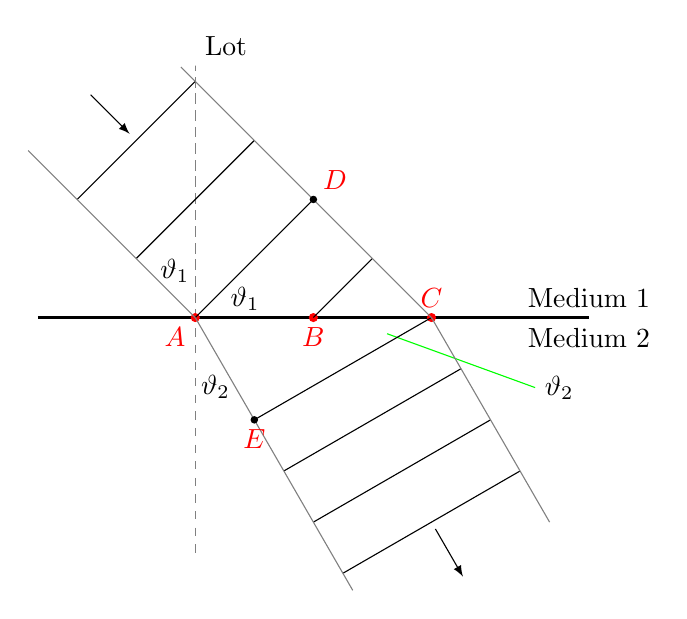
\begin{tikzpicture}
  \coordinate (a) at (1,0);
  \coordinate (b) at (2.5,0);
  \coordinate (c) at (4,0);
  % boundary
  \draw[thick] (-1,0) -- +(7,0) node[above] {Medium $1$} node[below] {Medium $2$};
  % plumb
  \draw[gray,dashed] (a) -- +(0,3.2) node[above right,black] {Lot} -- +(0,-3);
  \centerarc[gray](a)(90:135:1);
  \node[below] at ($(a)+(105:1)+(0,-0.1)$) {$\vartheta_1$};
  \centerarc[gray](a)(0:45:1);
  \node[left] at ($(a)+(20:1)+(0,-0.1)$) {$\vartheta_1$};
  \centerarc[gray](a)(-60:-90:1.2);
  \node[above] at ($(a)+(-75:1.3)+(-0.08,0.1)$) {$\vartheta_2$};
  \centerarc[gray](c)(180:210:1.2);
  \draw[green] ($(c)+(200:0.6)$) -- +(-20:2) node[right,black] {$\vartheta_2$};
  % elementary wave
  \draw[fill,red] (a) circle (0.05) node[below left] {$A$};
  \centerarc[blue](a)(180:360:0.5*3);
  % elementary wave
  \draw[fill,red] (b) circle (0.05) node[below] {$B$};
  \centerarc[blue](b)(180:360:0.5*1.5);
  % elementary wave
  \draw[fill,red] (c) circle (0.05) node[above] {$C$};
  % wave fronts
  \draw[] (a) -- +(45:0.707*3);
  \draw[] (b) -- +(45:0.707*1.5);
  \foreach \X in {1,2} { \draw ($(a)+(135:0.707*1.5*\X)$) -- +(45:0.707*3); };
  \foreach \X in {0,1,2,3} { \draw ($(c)+(-60:0.5*1.5*\X)$) -- +(-150:0.866*3); };
  % border
  \draw[gray] (a) -- +(135:3);
  \draw[gray] (a) -- +(-60:3+0.5*2);
  \draw[gray] (c) -- +(135:3+0.5*3);
  \draw[gray] (c) -- +(-60:3);
  % arrows
  \draw[->] ($(b)+(135:4)$) -- +(-45:0.7);
  \draw[->] ($(b)+(-60:3.1)$) -- +(-60:0.7);
  % points
  \coordinate (d) at ($(c)+(135:0.707*3)$);
  \coordinate (e) at ($(a)+(-60:1.5*0.5*2)$);
  \draw[fill] (d) circle (0.04);
  \draw[fill] (e) circle (0.04);
  \node[above right,red] at (d) {$D$};
  \node[below,red] at (e) {$E$};
\end{tikzpicture}
\end{document}
